\documentclass[conference]{IEEEtran}
\usepackage[T1]{fontenc}
\usepackage[utf8]{inputenc}
\usepackage{amsmath,amssymb,graphicx,booktabs,cite}
\usepackage{tikz,pgfplots}
\usetikzlibrary{arrows.meta,positioning,calc}
\pgfplotsset{compat=1.18}
\usepackage[hidelinks]{hyperref}
\urlstyle{same}
\definecolor{paperblue}{RGB}{36,75,101}
\definecolor{paperorange}{RGB}{173,98,58}
\newcommand{\recon}[1]{\raisebox{-.45\height}{\includegraphics[width=.67in]{images/#1.png}}}
\hyphenation{re-con-struc-tion bot-tle-neck Batch-Norm}

\begin{document}
\title{AR-TAPE for Split Learning in Medical Image Analysis}
\author{\IEEEauthorblockN{Bien Cao Cuong and Hoang Nguyen Tai Danh}
\IEEEauthorblockA{Faculty of Information Technology\\
University of Science and Technology, The University of Danang\\
Da Nang, Vietnam}}
\maketitle

\begin{abstract}
Split Learning transmits intermediate representations instead of raw images, but those representations can still support image reconstruction. We study AR-TAPE v1, which combines a fixed orthogonal bottleneck with capped adversarial reconstruction training at a ResNet-18 cut layer. On CIFAR-10, the transmitted representation is reduced from 65,536 to 2,048 values. Across three seeds, an adversarial coefficient of 0.25 yields full-test accuracy of $90.35\pm0.24\%$ and fresh-decoder SSIM of $0.2159\pm0.0029$ for an MLP-based attacker and $0.2014\pm0.0036$ for a convolutional attacker. Compared with the same bottleneck without adversarial training, SSIM decreases by 0.4918 and 0.3613 at a mean accuracy cost of approximately 0.70 percentage points. The original utility target of 92.7\% is not reached. Direct feature-space hijacking observations are also analyzed, but pilot compatibility and ambiguous run labels limit active-attack conclusions. Historical diagnostics update BatchNorm statistics on test images, so the stored results require confirmation with an isolated evaluation protocol. This study provides preliminary evidence of a reconstruction--utility trade-off against two tested decoders; it establishes neither formal privacy nor medical-image effectiveness. PCAM and HAM10000 experiments remain future work.
\end{abstract}

\begin{IEEEkeywords}
Split Learning, feature inversion, orthogonal projection, adversarial representation learning, reconstruction evaluation.
\end{IEEEkeywords}

\section{Introduction}
Hospitals may wish to train a shared image classifier while retaining patient images within their own institutions. Split Learning (SL) partitions a neural network between a client and a server: the client transmits an intermediate representation instead of the original image and receives gradients to update its local model~\cite{vepakomma2018split}. This workflow motivates the medical application considered here. However, keeping raw images local does not establish that the transmitted representation conceals their visual content. A decoder can learn to invert features, while an active server can manipulate training to make reconstruction easier~\cite{pasquini2021fsha}.

An empirical defense must therefore balance classification performance against reconstruction by attackers trained for the defended representation. A low reconstruction score for the adversary used during training is insufficient: another architecture or a newly optimized decoder may recover substantially more information. Dimensionality reduction introduces a related ambiguity. Although a projection is non-invertible over the complete feature space, the client may concentrate image information in the subspace that remains observable.

This paper studies AR-TAPE v1, an implementation combining a fixed global orthogonal bottleneck with capped adversarial reconstruction training. The name AR-TAPE denotes the broader research objective of absorption-resistant, task-aware perceptual encoding. In the evaluated version, task awareness arises from joint classification and adversarial optimization; the projection basis is random and fixed. Absorption resistance remains a hypothesis rather than an established property.

Our investigation addresses three questions. (1) Does adversarial training add value beyond the same bottleneck alone? (2) How do the trade-off and its variability change with the adversarial coefficient and decoder architecture? (3) What conclusions are supported by the available active-attack experiments? We make the following contributions within this project:
\begin{itemize}
\item An explicit formulation of the evaluated global-projection implementation, distinguishing it from a separate channel-projection module in the codebase.
\item A three-seed ablation at $\lambda\in\{0,0.25,0.5\}$ using fresh MLP and convolutional decoders, accompanied by source-derived tables and paired reconstruction examples.
\item An analysis of active-attack results and evaluation validity, including incompatible metric scopes, ambiguous run labels, and test-time BatchNorm updates.
\end{itemize}
The experiments are a CIFAR-10 proof of concept. They do not demonstrate clinical effectiveness, formal privacy, or superiority over the original LightSplit and ResSFL methods. The medical application is a motivation and a planned transfer setting.

\section{Related Work}
\subsection{Reconstruction and Active Attacks}
Feature inversion learns a decoder from representations to images. A fresh attacker is initialized after the client is fixed, testing whether the defense generalizes beyond its training-time adversary. A passive co-adapted decoder instead follows client updates without injecting attack gradients. Feature-Space Hijacking Attack (FSHA) changes this interaction: a malicious server uses a pilot representation, a decoder, and an alignment objective to influence the client's training~\cite{pasquini2021fsha}. These protocols reveal different failure modes and their scores should not be pooled into a single privacy claim.

\subsection{Representation Defenses}
ResSFL uses adversarial feature learning and resistance transfer in Split Federated Learning~\cite{li2022ressfl}. AR-TAPE shares the use of reconstruction adversaries but evaluates online alternating optimization on a separate testbed; no matched ResSFL reproduction is available. LightSplit uses orthogonal projections and lift-back operations~\cite{cihangiroglu2026lightsplit}. Our B7 baseline reproduces the fixed-projection component, not the full original method, which also considers U-shaped SL and Within-Class Compaction. Consequently, B7 is described as a LightSplit-style baseline.

NoPeek penalizes distance correlation between images and their representations~\cite{vepakomma2020nopeek}. Other internal baselines perturb features, gradients, spatial structure, or residual signals. These mechanisms act at different points in training. In particular, a batch-level gradient clipping implementation labeled ``DP-SGD'' does not by itself establish a differential privacy guarantee. Throughout this paper, image similarity and distance correlation are empirical proxies under specified tests, not privacy certificates.

\section{Method}
\subsection{Split Architecture and Threat Model}
We use ResNet-18~\cite{he2016resnet} adapted to $32\times32$ RGB images: a $3\times3$ stride-one stem replaces the original stem and max-pooling is removed. The client comprises the stem and Layer~1; the server comprises Layers~2--4, global average pooling, and a ten-class classifier. The cut activation contains $64\times32\times32=65{,}536$ values. Figure~\ref{fig:system} illustrates the transmitted representation and the reconstruction branch.

The passive server observes transmitted representations and knows the architecture, projection, and hyperparameters. Our fresh evaluation provides training image--feature pairs after freezing the client. It is thus a data-rich inversion test, not a simulation of every auxiliary-data constraint in deployment. Labels are available to the classification loss at the server; label privacy is outside this study. Active FSHA is evaluated separately because gradient manipulation exceeds the honest-but-curious threat model.

\begin{figure*}[t]
\centering
\begin{tikzpicture}[x=1cm,y=1cm,>=Latex,font=\footnotesize,
 module/.style={draw=blue!55!black,fill=blue!3,rounded corners=1pt,minimum height=1.0cm,align=center},
 flow/.style={->,thick,draw=blue!55!black},
 attack/.style={->,thick,draw=orange!75!black}]
\draw[fill=blue!2,draw=blue!20,rounded corners=3pt] (-.65,-.9) rectangle (5.85,1.43);
\draw[fill=gray!4,draw=gray!35,rounded corners=3pt] (6.05,-.9) rectangle (16.85,1.43);
\node[anchor=west,text=blue!55!black,font=\footnotesize\bfseries] at (-.4,1.17) {CLIENT / LOCAL IMAGES};
\node[anchor=west,text=gray!70!black,font=\footnotesize\bfseries] at (6.25,1.17) {SERVER / OBSERVED REPRESENTATION};
\node[inner sep=0] (x) at (0,0.15) {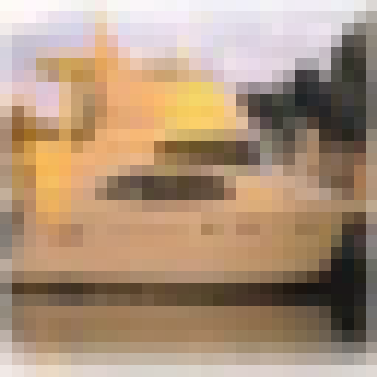
\includegraphics[width=.85cm]{images/x0.png}};
\node[below=.07cm of x] {$X\in\mathbb R^{3\times32\times32}$};
\node[module,minimum width=1.8cm] (client) at (1.9,.15) {ResNet-18 client\\Stem + Layer 1};
\node[module,minimum width=1.55cm] (project) at (4.72,.15) {Fixed projection\\$t=R^\top z$};
\node[module,minimum width=1.45cm] (lift) at (7.68,.15) {Fixed lift\\$\widetilde z=Rt$};
\node[module,minimum width=2.2cm] (server) at (10.4,.15) {ResNet-18 server\\Layers 2--4 + head};
\node[module,minimum width=1.5cm] (pred) at (13.4,.15) {Prediction\\$\widehat y$};
\node[align=center] at (15.6,.15) {Task loss\\$\mathcal L_{\rm cls}$};
\draw[flow] (x)--(client);
\draw[flow] (client)--(project);
\node at (3.35,.86) {$z$};
\node[font=\scriptsize] at (3.35,-.64) {$64\times32\times32$};
\draw[flow] (project)--(lift);
\node at (6.26,.86) {$t\in\mathbb R^{2048}$};
\draw[flow] (lift)--(server);
\draw[flow] (server)--(pred);
\draw[flow] (pred)--(15.05,.15);
\node[draw=orange!70!black,fill=orange!4,rounded corners=1pt,minimum height=.85cm,minimum width=3cm,align=center] (decoder) at (9,-1.8) {Reconstruction decoder $A_\phi$\\Training adversary or fresh attacker};
\draw[attack] (6.25,.15) |- (decoder.west);
\node[inner sep=0] (xh) at (12.2,-1.8) {
\includegraphics[width=.85cm]{images/mlp0.png}};
\draw[attack] (decoder)--(xh);
\node[below=.03cm of xh] {$\widehat X$};
\node[align=left,text=gray!80!black,anchor=west] at (-.4,-1.75) {Global bottleneck: $65{,}536\rightarrow2{,}048$\\$32{:}1$ fewer transmitted float values};
\node[align=left,text=orange!75!black,anchor=west] at (13.1,-1.8) {Reconstruction loss\\or post-hoc evaluation};
\end{tikzpicture}
\caption{Evaluated AR-TAPE v1. Only the projected representation $t$ crosses the cut. The client learns under task and adversarial losses, whereas $R$ is fixed. The pictured input and reconstruction are a real saved CIFAR-10 pair (fresh MLP, $\lambda=0.25$, seed 42); tensor labels describe architecture, not visualized activation values.}
\label{fig:system}
\end{figure*}


\subsection{Fixed Orthogonal Bottleneck}
Let $z=\operatorname{vec}(f_{\theta_c}(X))\in\mathbb{R}^{D}$ with $D=65{,}536$. A Gaussian matrix is orthonormalized by QR to obtain a fixed matrix $R\in\mathbb{R}^{D\times k}$, where $k=2{,}048$. Using column-vector notation,
\begin{equation}
 t=R^\top z,\qquad \widetilde z=Rt=RR^\top z,\qquad R^\top R=I_k.
 \label{eq:projection}
\end{equation}
The server reshapes $\widetilde z$ before classification. Since $\operatorname{rank}(RR^\top)=k<D$, the mapping discards components outside the column space of $R$. This algebraic fact does not show that $X$ is unrecoverable: the learned client can preserve image information within the transmitted subspace. The $\lambda=0$ ablation tests this limitation directly.

The evaluated implementation uses a global flattened projection stored as a fixed buffer. It is distinct from the channel-wise module elsewhere in the repository. Neither a learned projection basis nor an explicitly estimated pathology-specific task subspace is used in the reported v1 experiments.

\subsection{Capped Adversarial Optimization}
The adversary $A_\phi$ contains a learned lift $2{,}048\!\rightarrow\!512\!\rightarrow\!65{,}536$, BatchNorm, and four convolutional layers with channels $64\!\rightarrow\!128\!\rightarrow\!128\!\rightarrow\!64\!\rightarrow\!3$. It has approximately $35.1$ million trainable parameters. With normalized input $X_n$, its loss is
\begin{equation}
 \mathcal L_{\mathrm{rec}}=\operatorname{MSE}(A_\phi(t),X_n).
\end{equation}
Each minibatch uses one primary client forward pass. The adversary first minimizes $\mathcal L_{\mathrm{rec}}$ with $t$ detached. Its parameters are then frozen while the client and server minimize
\begin{align}
 \mathcal L_{\mathrm{cs}}&=\operatorname{CE}(\widehat y,y)-\lambda_e\min(\mathcal L_{\mathrm{rec}},c),\label{eq:objective}\\
 \lambda_e&=\lambda\min(1,e/10).
\end{align}
Here $e$ is the epoch and $c=1.5586$ is the measured mean squared energy of normalized CIFAR-10 images, corresponding to an all-zero reconstruction in normalized space. The adversarial term saturates at the cap. The classification gradient affects both model partitions; the reconstruction gradient affects the client through $t$. Freezing adversary parameters does not automatically put its BatchNorm layers in evaluation mode. Figure~\ref{fig:optimization} separates the two updates.

\begin{figure}[t]
\centering
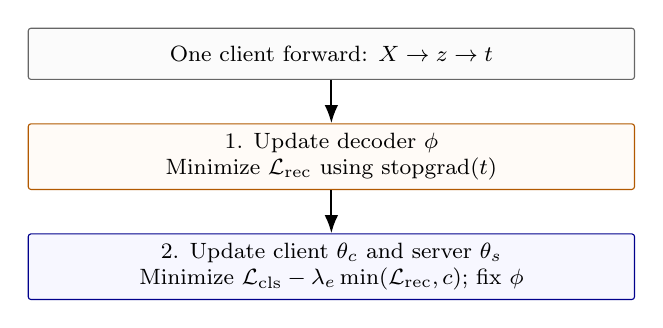
\begin{tikzpicture}[>=Latex,font=\footnotesize,node distance=.55cm,
 b/.style={draw=black!60,fill=gray!3,rounded corners=1pt,align=center,minimum width=7.7cm,minimum height=.65cm}]
\node[b] (forward) {One client forward: $X\rightarrow z\rightarrow t$};
\node[b,below=of forward,draw=orange!70!black,fill=orange!3] (adv) {1. Update decoder $\phi$\\Minimize $\mathcal L_{\rm rec}$ using $\operatorname{stopgrad}(t)$};
\node[b,below=of adv,draw=blue!55!black,fill=blue!3] (model) {2. Update client $\theta_c$ and server $\theta_s$\\Minimize $\mathcal L_{\rm cls}-\lambda_e\min(\mathcal L_{\rm rec},c)$; fix $\phi$};
\draw[->,thick] (forward)--(adv);
\draw[->,thick] (adv)--(model);
\end{tikzpicture}
\caption{Alternating minibatch updates. The reconstruction term changes the client representation; the server receives the task gradient. Freezing decoder parameters alone does not freeze its BatchNorm buffers.}
\label{fig:optimization}
\end{figure}


\subsection{Evaluation Attackers}
\textit{Fresh MLP} learns a $2{,}048\!\rightarrow\!512\!\rightarrow\!65{,}536$ lift followed by the four-layer convolutional decoder. \textit{Fresh Conv} uses the fixed transpose lift of the bottleneck and learns the convolutional decoder. The client is frozen in evaluation mode during these attack fits. Both attackers train for 30 epochs using Adam with initial learning rate $10^{-3}$ and cosine decay. For the main $\lambda=0.25$ group, all three stored best epochs equal the final epoch, 30. These two architectures do not represent every possible attacker.

The direct FSHA experiment uses 25,000 training images to fit a pilot and another 25,000 for hijacking. It starts from trained client/server checkpoints and updates the client with classification plus a scaled hijacking objective for 30 epochs, using gradient scales $g_s\in\{1,5\}$. The pilot is not constrained to the defended projection subspace. This protocol differs from historical baseline attacks in initialization and task-gradient mixing, limiting causal comparisons across methods.

\section{Experimental Setup}
\subsection{Data and Training}
CIFAR-10~\cite{krizhevsky2009cifar} contains 50,000 training images and 10,000 test images across ten classes. Training uses random cropping with padding four, horizontal flipping, and channel normalization with mean $(0.4914,0.4822,0.4465)$ and standard deviation $(0.2023,0.1994,0.2010)$. Test images are only normalized. A seed-fixed 2,000-image subset of the test set, denoted \emph{fast 2k}, is used for diagnostic evaluations; it must be distinguished from the full 10k test set.

The main models train for 100 epochs with batch size 128, SGD, initial learning rate $0.1$, momentum $0.9$, weight decay $5\times10^{-4}$, and a cosine schedule. The adversarial coefficient is warmed up for ten epochs. We evaluate $\lambda=0,0.25,0.5$ using seeds 42, 7, and 2024; $\lambda=0.1$ has only seed 42. The same-architecture $\lambda=0$ model is the most direct control for the adversarial term. Historical baselines generally have one seed and differ in training schedules or attack checkpoint selection.

\subsection{Metrics and Aggregation}
Classification utility is measured by top-1 accuracy. Reconstruction is measured by PSNR, SSIM~\cite{wang2004ssim}, and LPIPS~\cite{zhang2018lpips}. Higher PSNR/SSIM and lower LPIPS indicate greater similarity to the original. PSNR and SSIM are evaluated after denormalization and clamping to $[0,1]$. For the v1 fresh attacks, they use the full 10k test set; available LPIPS uses fast 2k only. Direct FSHA reports full-test accuracy but fast-2k reconstruction metrics.

Distance correlation (dCor)~\cite{szekely2007dcor} is taken from the final ordinary-training diagnostic, averaged over the first ten batches of the fast subset. It is neither mutual information nor a formal privacy guarantee. Multi-seed results are means and sample standard deviations ($n-1$ denominator). They describe variation between runs on one test set, not a confidence interval for clinical generalization.

We retain the original project criteria: accuracy $\geq92.7\%$, PSNR $<15$~dB, and SSIM $<0.3$ against the required attackers. LPIPS $>0.2$ is an additional perceptual target. These are engineering goals, not universal safety thresholds. We do not lower the utility target after inspecting results. Hyperparameter exploration on the test set and BatchNorm-state contamination further limit the interpretation, as discussed in Section~\ref{sec:limitations}.

\section{Results}
\subsection{Comparison with Internal Baselines}
\begin{table*}[t]
\centering
\caption{Available internal baseline comparisons. Accuracy and fresh SSIM use the full 10k test set.}
\label{tab:baselines}
\footnotesize
\setlength{\tabcolsep}{4pt}
\begin{tabular}{@{}lcccc@{}}
\toprule
Method & Seeds & Accuracy (\%) $\uparrow$ & Fresh MLP SSIM $\downarrow$ & Fresh Conv SSIM $\downarrow$ \\
\midrule
B0: Vanilla SL & 1 & 94.71 & --- & 0.9955 \\
B7: Fixed projection, $k=512$ & 1 & 88.54 & 0.4394 & 0.2632 \\
B7: Fixed projection, $k=1{,}024$ & 1 & 91.53 & 0.5461 & 0.3597 \\
B7: Fixed projection, $k=2{,}048$ & 1 & 92.73 & --- & --- \\
B8: Original min--max & 1 & 92.38 & 0.4580 & 0.7652 \\
B8: Stabilized min--max & 1 & 88.98 & 0.2621 & 0.6431 \\
\textbf{AR-TAPE v1}, $k=2{,}048$, $\lambda=0.25$ & 3 & $90.35\pm 0.24$ & $0.2159\pm 0.0029$ & $0.2014\pm 0.0036$ \\
\bottomrule
\end{tabular}
\par\vspace{2pt}\begin{minipage}{\linewidth}\footnotesize Historical methods differ in schedules and attacker checkpoint selection. B7 is a partial LightSplit-style implementation. Dashes indicate missing standardized fresh measurements, not privacy protection. Lower SSIM is the defense objective, not a general privacy certificate.\end{minipage}
\end{table*}

Table~\ref{tab:baselines} compares available standardized fresh evaluations. A missing entry indicates an unavailable measurement, not an unsuccessful attacker. B7 with $k=2{,}048$ has an older decoder result (SSIM $0.5138$), but no matched standardized fresh MLP/Conv pair; we do not insert that value into the Conv column. B8 attack scripts selected checkpoints using test reconstruction, although the records used here have their best epoch at the final epoch, 30. These protocol differences preclude a controlled ranking of all baselines.

The stabilized B8 model illustrates attacker dependence: fresh MLP reaches SSIM $0.2621$, whereas fresh Conv reaches $0.6431$. On the common fast-2k scope, the Conv score exceeds that of the training-time adversary by $G=0.2948$. This gap shows incomplete coverage by the internal adversary; it does not uniquely establish that the server absorbed an inverse mapping. Decoder architecture and optimization remain alternative explanations.

Other stored controls reinforce the need for adaptive evaluation. NoPeek at $\alpha=1$ attains dCor near $0.0479$ while reconstruction SSIM remains $0.9038$. A residual-autoencoder defense increases from SSIM $0.7129$ with an old decoder to $0.9976$ after system/decoder retraining. Block scrambling is inverted by a learned MLP at SSIM $0.9252$. These are contextual observations from historical protocols rather than matched causal comparisons with v1.

\subsection{Does Adversarial Training Add Value?}
\begin{table*}[t]
\centering
\caption{Coefficient ablation with the same fixed $k=2{,}048$ bottleneck. Values are mean $\pm$ sample SD.}
\label{tab:ablation}
\footnotesize
\setlength{\tabcolsep}{4pt}
\begin{tabular}{@{}cccccc@{}}
\toprule
$\lambda$ & Seeds & Accuracy 10k (\%) $\uparrow$ & MLP SSIM 10k $\downarrow$ & Conv SSIM 10k $\downarrow$ & dCor \\
\midrule
0.00 & 3 & $91.05\pm 0.36$ & $0.7077\pm 0.0059$ & $0.5627\pm 0.0065$ & $0.5717\pm 0.0091$ \\
0.10 & 1 & $90.37$ & $0.2261$ & $0.1938$ & $0.3020$ \\
0.25 & 3 & $90.35\pm 0.24$ & $0.2159\pm 0.0029$ & $0.2014\pm 0.0036$ & $0.2876\pm 0.0077$ \\
0.50 & 3 & $89.41\pm 0.50$ & $0.2425\pm 0.0144$ & $0.2315\pm 0.0048$ & $0.2404\pm 0.0224$ \\
\bottomrule
\end{tabular}
\par\vspace{2pt}\begin{minipage}{\linewidth}\footnotesize dCor is taken only from ordinary-training diagnostics on fast 2k, not post-FSHA records. The $0.1$ group has one seed; its variability is unknown.\end{minipage}
\end{table*}

\begin{figure*}[t]
\centering
\begin{tikzpicture}
\begin{axis}[
 name=accuracy,width=.47\textwidth,height=5.0cm,
 font=\footnotesize,label style={font=\footnotesize},
 xmin=-.025,xmax=.525,ymin=88,ymax=93.2,
 xlabel={Adversarial coefficient $\lambda$},ylabel={Accuracy on 10k (\%)},
 xtick={0,.1,.25,.5},xticklabels={0,0.1,0.25,0.5},
 ytick={88,89,90,91,92,93},grid=major,grid style={gray!18},
 axis lines=left,legend style={draw=none,font=\scriptsize,at={(.98,.97)},anchor=north east}]
\addplot[only marks,mark=*,mark size=1.2pt,gray!75] table[x=lambda,y=acc]{data/seeds.dat};
\addlegendentry{Individual seeds}
\addplot[paperblue,thick,mark=*,mark size=2.1pt,error bars/.cd,y dir=both,y explicit]
 table[x=lambda,y=acc,y error=accsd]{data/sweep.dat};
\addlegendentry{Mean $\pm$ SD}
\addplot[paperorange,dashed,domain=-.025:.525] {92.7};
\addlegendentry{Original target: 92.7\%}
\end{axis}
\begin{axis}[
 at={(accuracy.east)},anchor=west,xshift=1.35cm,
 width=.47\textwidth,height=5.0cm,
 font=\footnotesize,label style={font=\footnotesize},
 xmin=-.025,xmax=.525,ymin=0,ymax=.8,
 xlabel={Adversarial coefficient $\lambda$},ylabel={Fresh SSIM on 10k},
 xtick={0,.1,.25,.5},xticklabels={0,0.1,0.25,0.5},
 ytick={0,.2,.4,.6,.8},grid=major,grid style={gray!18},
 axis lines=left,legend style={draw=none,font=\scriptsize,at={(.98,.97)},anchor=north east}]
\addplot[forget plot,only marks,mark=*,mark size=1.2pt,paperblue!45] table[x=lambda,y=mlp]{data/seeds.dat};
\addplot[paperblue,thick,mark=*] table[x=lambda,y=mlp]{data/sweep.dat};
\addlegendentry{Fresh MLP}
\addplot[forget plot,only marks,mark=square*,mark size=1.2pt,paperorange!45] table[x=lambda,y=conv]{data/seeds.dat};
\addplot[paperorange,thick,mark=square*] table[x=lambda,y=conv]{data/sweep.dat};
\addlegendentry{Fresh Conv}
\addplot[gray,dashed,domain=-.025:.525] {.3};
\addlegendentry{Project SSIM target: 0.3}
\end{axis}
\end{tikzpicture}
\caption{Coefficient sweep computed from source records. Small markers show individual seeds; large markers show group means. Accuracy error bars are sample standard deviations. The $\lambda=0.1$ group contains one seed. Lines guide the eye; dashed references are project criteria, not formal privacy boundaries. Larger $\lambda$ does not monotonically improve fresh reconstruction resistance.}
\label{fig:sweep}
\end{figure*}

With no adversarial term, the same bottleneck yields accuracy $91.05\pm0.36\%$, but fresh MLP and Conv still recover SSIM $0.7077\pm0.0059$ and $0.5627\pm0.0065$, respectively (Table~\ref{tab:ablation}). Thus, reducing feature dimensionality alone is insufficient against these decoders.

At $\lambda=0.25$, the corresponding scores decrease to $0.2159\pm0.0029$ and $0.2014\pm0.0036$, while accuracy decreases by approximately $0.70$ percentage points to $90.35\pm0.24\%$. The absolute SSIM reductions are $0.4918$ and $0.3613$. This ablation provides the clearest evidence in the current experiments for the contribution of the adversarial term.

Increasing $\lambda$ from $0.25$ to $0.5$ reduces accuracy further while increasing both fresh SSIM scores. The observed relationship is therefore not monotonic (Fig.~\ref{fig:sweep}). The single-seed $\lambda=0.1$ result also remains competitive, so the present sweep does not establish $0.25$ as a generally optimal coefficient. A separate validation set is required for operating-point selection.

Recomputing dCor from ordinary training gives $0.5717\pm0.0091$ for $\lambda=0$ and $0.2404\pm0.0224$ for $\lambda=0.5$. Earlier aggregate values $0.7219$ and $0.4348$ belonged to post-FSHA states and are excluded. Moreover, $\lambda=0.5$ has lower dCor than $0.25$ but higher fresh SSIM. dCor does not rank reconstruction difficulty in the same way as the two evaluated decoders.

\subsection{Main Operating Point and Visual Evidence}
\begin{table}[t]
\centering
\caption{Fresh reconstruction at $\lambda=0.25$ (three seeds).}
\label{tab:reconstruction}
\footnotesize
\setlength{\tabcolsep}{4pt}
\begin{tabular}{@{}lccc@{}}
\toprule
Attacker & SSIM 10k $\downarrow$ & PSNR 10k (dB) $\downarrow$ & LPIPS 2k $\uparrow$ \\
\midrule
MLP & $0.2159\pm 0.0029$ & $13.39\pm 0.13$ & $0.2678\pm 0.0078$ \\
Conv & $0.2014\pm 0.0036$ & $12.48\pm 0.01$ & $0.1881\pm 0.0012$ \\
\bottomrule
\end{tabular}
\par\vspace{2pt}\begin{minipage}{\linewidth}\footnotesize Arrows indicate the defense objective. LPIPS uses fast 2k only. The Conv value does not reach the additional $>0.2$ perceptual target.\end{minipage}
\end{table}

\begin{figure*}[t]
\centering
\setlength{\tabcolsep}{2pt}
\begin{tabular}{@{}l*{6}{c}@{}}
Original $X$ & \recon{x0}&\recon{x1}&\recon{x2}&\recon{x3}&\recon{x4}&\recon{x5}\\\noalign{\vskip 3pt}
$\lambda=0$, MLP & \recon{lam00}&\recon{lam01}&\recon{lam02}&\recon{lam03}&\recon{lam04}&\recon{lam05}\\\noalign{\vskip 3pt}
$\lambda=0.25$, MLP & \recon{mlp0}&\recon{mlp1}&\recon{mlp2}&\recon{mlp3}&\recon{mlp4}&\recon{mlp5}\\\noalign{\vskip 3pt}
$\lambda=0.25$, Conv & \recon{conv0}&\recon{conv1}&\recon{conv2}&\recon{conv3}&\recon{conv4}&\recon{conv5}
\end{tabular}
\caption{Paired examples from the first six columns of saved seed-42 grids. Original-image rows were verified to be pixel-identical before combining the panels. The $\lambda=0.25$ MLP and Conv checkpoints both have best epoch equal to final epoch 30. Reconstructions are actual saved outputs, without generated or enhanced image content. Visible residual structure cautions against interpreting low similarity as the absence of all semantic leakage.}
\label{fig:reconstructions}
\end{figure*}

At $\lambda=0.25$, both fresh attackers satisfy the project's PSNR and SSIM goals (Table~\ref{tab:reconstruction}). However, Conv LPIPS is $0.1881\pm0.0012$, below the additional target $0.2$. The paired examples in Fig.~\ref{fig:reconstructions} show reduced fidelity relative to the $\lambda=0$ model, but residual colors and coarse structure remain visible. Low average similarity therefore does not demonstrate the absence of sensitive semantic information.

The mean accuracy is $4.36$ percentage points below the historical vanilla result, $94.71\%$, and $2.35$ points below the retained utility target. The complete PoC criteria are not met. Relative to the previous v0 result of $87.34\%$ on one seed, v1 improves observed utility and adds multi-seed evidence. That comparison also changes bottleneck width, projection type, lifting, and scheduling; it cannot isolate the contribution of any one change.

\subsection{Direct FSHA and Its Interpretation}
\begin{table}[t]
\centering
\caption{Direct FSHA at epoch 30. Reconstruction uses fast 2k.}
\label{tab:fsha}
\footnotesize
\setlength{\tabcolsep}{4pt}
\begin{tabular}{@{}cccccc@{}}
\toprule
$\lambda$ & $g_s$ & $n$ & Acc. 10k (\%) & SSIM 2k & PSNR (dB) \\
\midrule
0.0 & 1 & 1 & $87.27$ & $0.0251$ & $10.63$ \\
0.0 & 5 & 1 & $84.20$ & $0.0402$ & $11.86$ \\
$0.25^{*}$ & 1 & 3 & $87.61\pm 0.29$ & $0.0236\pm 0.0108$ & $10.55\pm 0.19$ \\
$0.25^{*}$ & 5 & 3 & $84.94\pm 1.07$ & $0.0394\pm 0.0102$ & $11.55\pm 0.22$ \\
0.5 & 1 & 1 & $86.98$ & $0.0241$ & $10.51$ \\
0.5 & 5 & 1 & $83.44$ & $0.0377$ & $11.66$ \\
\bottomrule
\end{tabular}
\par\vspace{2pt}\begin{minipage}{\linewidth}\footnotesize $^{*}$Directory-defined group: stored run labels say $\lambda=0.1$. Checkpoint provenance is not conclusively established. These observations do not prove active-attack resistance.\end{minipage}
\end{table}

Table~\ref{tab:fsha} reports epoch-30 direct-FSHA observations. The group marked $0.25^{*}$ is identified by its output directory. All three stored JSON files instead label their coefficient as $0.1$. Inspection of the runner shows that checkpoint paths are constructed from the current coefficient but the child process is not passed the coefficient-label argument, leaving its default at $0.1$. This is consistent with a metadata error, but the files do not retain checkpoint hashes that would establish run provenance conclusively. We retain the directory-defined group conditionally and do not treat it as definitive evidence of FSHA resistance at $\lambda=0.25$.

Crucially, $\lambda=0$ also yields very low FSHA SSIM ($0.0402$ at $g_s=5$), despite fresh MLP SSIM around $0.7077$. A weak reconstruction result for this active attack does not imply that the representation lacks recoverable information. The unconstrained pilot and the lifted defended representation may be mismatched; insufficient attack optimization is another possibility. These are hypotheses requiring targeted tests. A pilot fitted directly to the defended bottleneck, as well as additional adaptive inversion attacks, is needed before drawing a broad robustness conclusion.

The directory-defined three-seed group attains post-hijacking accuracy $84.94\pm1.07\%$ at $g_s=5$. This is the model state after attack training. It must not be combined with the pre-attack accuracy $90.35\%$ as if both measured the same model. Matching gradient scale and attack epochs alone also does not remove differences in initialization, data usage, and task-gradient mixing across historical baseline protocols.

\section{Discussion and Limitations}
\label{sec:limitations}
\subsection{What the Evidence Supports}
The same-architecture ablation supports combining a restricted transmission subspace with adversarial reconstruction training to reduce the fidelity of two tested fresh decoders. The B8 counterexample demonstrates why a single in-training adversary is an insufficient evaluation. Neither observation establishes a formal privacy guarantee or identifies server absorption as the unique causal mechanism. The ``absorption-resistant'' component of the project name remains a research objective.

\subsection{Evaluation-State Contamination}
A significant validity limitation is present in the historical training scripts. Diagnostic accuracy and reconstruction evaluations call the client in training mode on test images without fully restoring BatchNorm running means and variances. Disabling gradients does not prevent these buffers from updating. Such diagnostics are repeated during training, and a final full-test training-mode pass occurs before checkpoint saving. Consequently, the saved checkpoint can contain test-influenced normalization statistics, and the checkpoint used by fresh attackers need not share the BatchNorm state used in the preceding evaluation-mode accuracy measurement.

We report the stored observations without claiming that they constitute an independent, untouched test evaluation. Three seeds characterize variability within this procedure but do not remove its systematic bias. Confirmation requires preserving/restoring the complete model state for diagnostics or using cloned models, selecting hyperparameters on validation data, and evaluating one fixed checkpoint in evaluation mode. No such corrected rerun is available in the audited results. This issue is a priority before external publication.

\subsection{Computational Cost and Scope}
The transmitted float32 feature payload decreases from 256~KiB to 8~KiB per example, a $32{:}1$ reduction in value count. This is not a measured end-to-end network or latency speedup. The dense $65{,}536\times2{,}048$ projection contains $134{,}217{,}728$ elements, requiring 512~MiB per float32 copy; the server stores another lift copy. The 35.1M-parameter adversary and optimizer state add substantial training cost. No matched runtime or memory profiling supports an edge-efficiency claim.

The evidence is limited to one dataset, one cut layer, and a small attacker family. Most historical baselines use one seed. No matched ResSFL reproduction, formal differential privacy analysis, membership inference, attribute inference, or label-privacy evaluation is available. A comprehensive co-adapted v1 evaluation is also absent from the evidence summarized here. Similarity metrics cannot substitute for these tests.

\subsection{Transfer to Medical Images}
The codebase now contains medical dataset loaders, PCAM/HAM10000 configurations, and clinical metrics, but no medical experiment outputs were found. PCAM~\cite{veeling2018pcam} and HAM10000~\cite{tschandl2018ham} are planned transfer datasets, not validated applications in this paper. Their evaluation should use suitable official partitions and lesion-/patient-grouped splitting where available, with sensitivity/specificity thresholds selected only on validation data. The current optional Youden-threshold fallback on the evaluated set must not be used for final test reporting. Resizing all images to $32\times32$ also requires a resolution ablation because clinically relevant detail may be lost.

\subsection{Reproducibility}
We audited 85 stored JSON files at repository snapshot \texttt{be737ce33b21} on October~25,~2026; models were not retrained for this manuscript. Tables and plots are recalculated from primary records rather than copied from annotated summary figures. Missing values remain missing. The source package includes a machine-readable results snapshot and figure provenance.

Historical filenames still contain ``v0''; architecture is identified from fixed-bottleneck and lifting metadata. The source snapshot lists the utility-sweep and scheduler/cosine record paths. Newly unified entrypoints have not reproduced the complete archived protocol, including FSHA, and are not the source of these numbers.

\section{Conclusion}
AR-TAPE v1 combines a fixed $k=2{,}048$ orthogonal bottleneck with capped adversarial reconstruction training. On three CIFAR-10 seeds, $\lambda=0.25$ achieves accuracy $90.35\pm0.24\%$ and fresh SSIM $0.2159\pm0.0029$ (MLP) and $0.2014\pm0.0036$ (Conv). Relative to the same bottleneck without adversarial training, reconstruction fidelity decreases substantially at a mean accuracy cost of about $0.70$ percentage points. This is evidence for an empirical trade-off against the tested decoders, not a general privacy result.

Utility remains below the original PoC target. Test-time BatchNorm contamination, FSHA provenance and pilot compatibility, validation-based model selection, and stronger adaptive attacks must be addressed before stronger claims are justified. Medical-image validation remains future work.


\bibliographystyle{IEEEtran}
\bibliography{references}
\end{document}
